\renewcommand*{\arraystretch}{1.5}
\noindent\begin{tabularx}{17cm}{|p{1.95cm}|X|}
	\hline
	number      & 18                                                          \\ \hline
	title       & How many persons have a given number of posts                                                           \\ \hline
	\multicolumn{2}{|c|}{ 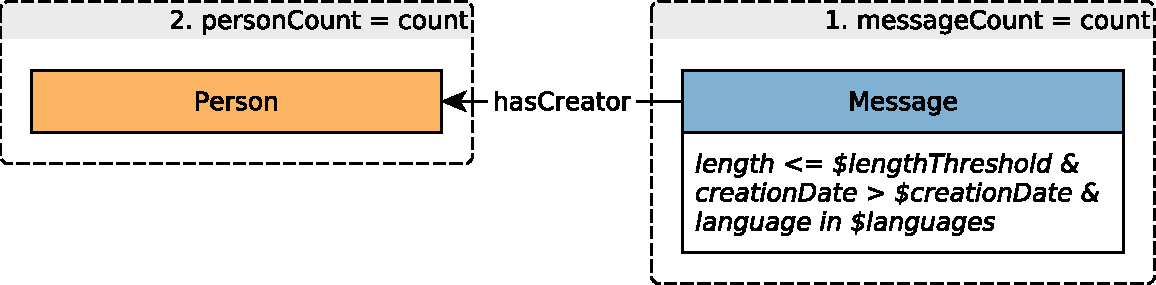
\includegraphics[scale=\patternscale,margin=0cm .2cm]{patterns/q18}} \\ \hline
	description & For each Person, count the number of Messages (Posts \& Comments) they
made.

Only consider messages with:

\begin{itemize}
\tightlist
\item
  length below the \texttt{lengthThreshold}
\item
  creationDate after \texttt{creationDate} (TODO - is after exclusive or
  inclusive, does it allow equality?)
\item
  any of the given \texttt{languages} (TODO - only Posts have a
  language, messages do not)
\end{itemize}
 \\ \hline
	
	group by       &
	\multicolumn{1}{>{\raggedright}X|}{
		\varname{messageCount}
		}\\ \hline
	
	parameters  &
	\renewcommand*{\arraystretch}{1.0}
	\vspace{-1.8ex}{\begin{tabularx}{14.2cm}{|c|l|p{2cm}|Y|} \hline
	\cellcolor{black!70} \color{white} $\mathsf{ 1 }$ & \varname{creationDate} & \cellcolor{gray!20} \vartype{Date} & \\ \hline
	\cellcolor{black!70} \color{white} $\mathsf{ 2 }$ & \varname{lengthThreshold} & \cellcolor{gray!20} \vartype{TODO (32bitInteger?)} & \\ 
	\end{tabularx}} \\ \hline
	result      &
	\renewcommand*{\arraystretch}{1.0}
	\vspace{-1.8ex}{\begin{tabularx}{14.2cm}{|c|l|p{2cm}|Y|} \hline
	\cellcolor{black!70} \color{white} $\mathsf{ 1 }$ & \varname{messageCount} & \cellcolor{gray!20} \vartype{32bitInteger} &number of messages created \\ \hline
	\cellcolor{black!70} \color{white} $\mathsf{ 2 }$ & \varname{personCount} & \cellcolor{gray!20} \vartype{32bitInteger} &the number of Persons with `messageCount` messages \\ 
	\end{tabularx}} \\ \hline
	sort        &
	\renewcommand*{\arraystretch}{1.0}
	\vspace{-1.8ex}{\begin{tabular}{|c|l|c|} \hline
	\cellcolor{black!70} \color{white} $\mathsf{ 1 }$ & \varname{personCount} & \cellcolor{gray!20} $\desc$ \\ 
	\end{tabular}} \\ \hline
	choke points        &
	\multicolumn{1}{>{\raggedright}X|}{
		\chokepoint{1.1}, 
		\chokepoint{1.2}, 
		\chokepoint{1.6}, 
		\chokepoint{3.2}, 
		\chokepoint{4.2}, 
		\chokepoint{4.3}
		}\\ \hline
\end{tabularx}
\clearpage